\lstinputlisting[language=bash,basicstyle=\small]{python_codes/fieldstone_61/keywords.ascii}

\begin{center}
Code at \url{https://github.com/cedrict/fieldstone/tree/master/python_codes/fieldstone_61}
\end{center}

\par\noindent\rule{\textwidth}{0.4pt}
%%%%%%%%%%%%%%%%%%%%%%%%%%%%%%%%%%%%%%%%%%%%%%%%%%%%%%%%%%%%%%%%%%%%%%%%%%%%%%%%%%%%%%%%%%%%

\paragraph{Simple Newtonian Poiseuille flow} The analytical solution to this flow has been derived 
in Section~\ref{MMM-ss:poiseuille}.
We set $p_{left}=10^9$, $p_{right}=0$, $L_x=L_y=100$km, $\eta_0=10^{25}$, so 
\[
\Pi=\frac{p_{right}-p_{left}}{L_x}=-10^4 <0
\]
The $p_{left}$ value is prescribed on the left (see Section~\ref{MMM-ss:openbc}) while 
nothing is prescribed on the right. No slip boundary conditions are 
prescribed on the top and bottom.

We see that we recover the analytical solution for velocity and strainrate:
\begin{center}
\includegraphics[width=7.8cm]{python_codes/fieldstone_61/results/poiseuille/velocity}
\includegraphics[width=7.8cm]{python_codes/fieldstone_61/results/poiseuille/exy}
\end{center}

\begin{center}
\includegraphics[width=5cm]{python_codes/fieldstone_61/results/poiseuille/vel}
\includegraphics[width=5cm]{python_codes/fieldstone_61/results/poiseuille/press}
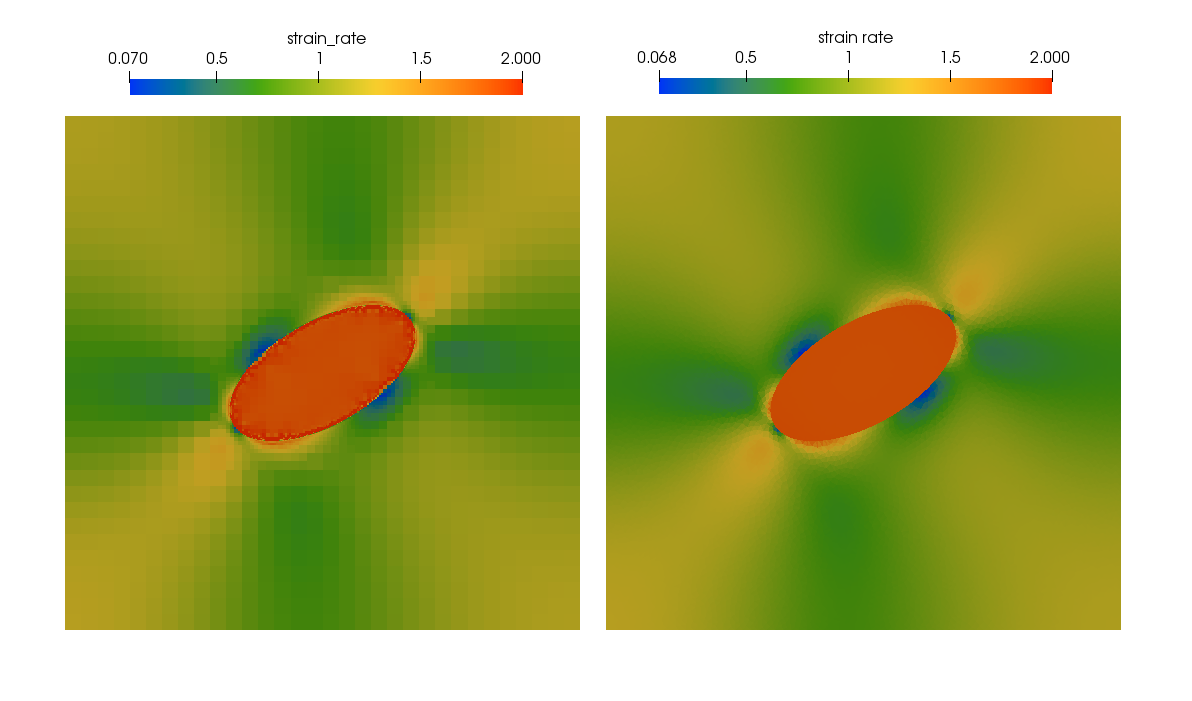
\includegraphics[width=5cm]{python_codes/fieldstone_61/results/poiseuille/sr}
\end{center}

\paragraph{Poiseuille flow with H-B rheology - $n=1$} 
The analytical solution to this flow has been derived in Section~\ref{MMM-ss:HBflow}.
In this case we have 
\[
\eta_{HB}
=
\left\{
\begin{array}{lc}
\eta_0 & \dot{\varepsilon}_e\leq \dot{\varepsilon}_0 \\
K  + \frac{\tau_0}{\dot{\varepsilon}_e}  
& \dot{\varepsilon}_e\geq \dot{\varepsilon}_0 
\end{array}
\right.
\]
and the limiting viscosity $\eta_0$ is such that 
\[
\eta_0 = K  + \frac{\tau_0}{\dot{\varepsilon}_0}  
\]

\begin{center}
\includegraphics[width=7.8cm]{python_codes/fieldstone_61/results/n_1/velocity.pdf}
\includegraphics[width=7.8cm]{python_codes/fieldstone_61/results/n_1/exy.pdf}\\
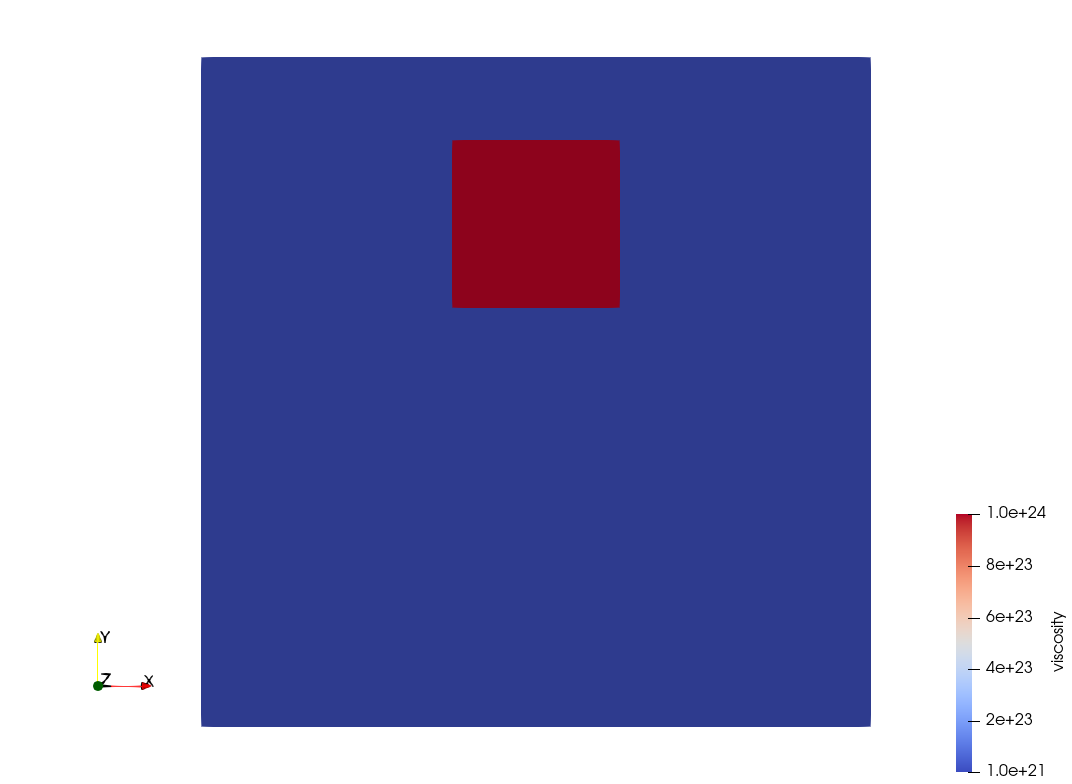
\includegraphics[width=7.8cm]{python_codes/fieldstone_61/results/n_1/eta.pdf}
\includegraphics[width=7.8cm]{python_codes/fieldstone_61/results/n_1/press.pdf}\\
\includegraphics[width=7.8cm]{python_codes/fieldstone_61/results/n_1/nonlinear_conv.pdf}
\end{center}

\begin{center}
\includegraphics[width=7.8cm]{python_codes/fieldstone_61/results/n_1/vel.png}
\includegraphics[width=7.8cm]{python_codes/fieldstone_61/results/n_1/exy.png}\\
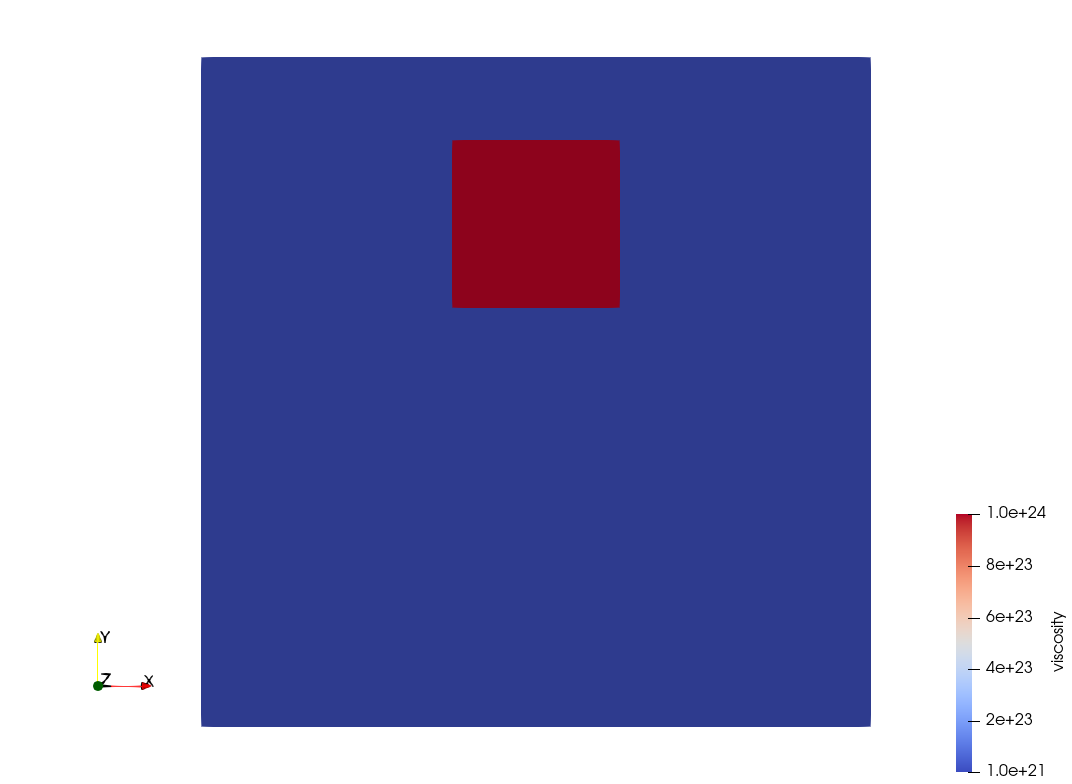
\includegraphics[width=7.8cm]{python_codes/fieldstone_61/results/n_1/eta.png}
\includegraphics[width=7.8cm]{python_codes/fieldstone_61/results/n_1/press.png}
\end{center}





